
% \documentclass{beamer}
\documentclass[aspectratio=169]{beamer}
% Theme settings
\usetheme{Madrid}
\usecolortheme{default}
\useinnertheme{rectangles}
\useoutertheme{miniframes}
\setbeamertemplate{navigation symbols}{}
\setbeamertemplate{caption}[numbered]
% Required packages
\usepackage{graphicx}
\usepackage{booktabs}
\usepackage{xcolor}
\usepackage{hyperref}
\usepackage{tikz}
\usepackage{amsmath}
\usepackage[most]{tcolorbox} % Load with 'most' option for more features
\usepackage{multicol}
\usepackage{listings}
\usepackage{array}
\lstset{
  basicstyle=\footnotesize\ttfamily,
  breaklines=true,
  frame=single,
  showstringspaces=false,
  keywordstyle=\color{blue},
  commentstyle=\color{green!60!black},
  stringstyle=\color{purple},
}

\title{Hardware Trojan Detection Using Graph Neural Networks}
\subtitle{AST-based Analysis with GCN Architecture}
\author{Md Omar Faruque}
\date{\today}

\begin{document}

\begin{frame}
\titlepage
\end{frame}

\begin{frame}
\frametitle{Outline}
\tableofcontents
\end{frame}

\section{Introduction}

\begin{frame}
\frametitle{Hardware Trojans: A Significant Threat}
\begin{itemize}
    \item \textbf{Hardware Trojans}: Malicious modifications to circuit designs
    \item Often inserted during third-party manufacturing or through IP cores
    \item Can lead to:
    \begin{itemize}
        \item Information leakage
        \item Denial of service
        \item Functional changes
    \end{itemize}
    \item \textbf{Challenge}: Detection is difficult at RTL level
    \item \textbf{Our approach}: Use Graph Neural Networks on code representations
\end{itemize}
\end{frame}

\begin{frame}
\frametitle{Verilog RTL \& Graph Representations}

\textbf{Abstract Syntax Tree (AST)}
\begin{itemize}
    \item Represents code structure
    \item Language constructs as nodes
    \item Parent-child relationships
    \item Captures programming patterns
\end{itemize}

\textbf{Our approach}: Using AST representation for more effective trojan detection
\end{frame}

\section{AST Generation}

\begin{frame}
\frametitle{What is an Abstract Syntax Tree (AST)?}
\begin{columns}
\column{0.6\textwidth}
\textbf{Simple definition:}
\begin{itemize}
    \item AST is a tree representation of code's structure
    \item Every line of code becomes a branch in the tree
    \item Similar to how sentences have grammar structure
\end{itemize}

\textbf{Advantages for trojan detection:}
\begin{itemize}
    \item Preserves programming patterns
    \item Shows suspicious control flow
    \item Captures language-specific features
\end{itemize}

\column{0.4\textwidth}
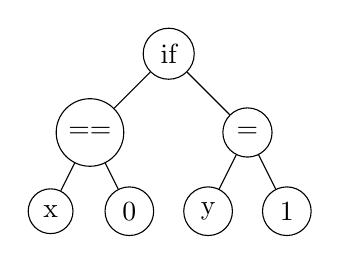
\begin{tikzpicture}[
    level distance=1cm,
    level 1/.style={sibling distance=2cm},
    level 2/.style={sibling distance=1cm},
    every node/.style={draw, circle, minimum size=0.5cm}
]
\node {if}
    child {node {==} 
        child {node {x}}
        child {node {0}}
    }
    child {node {=}
        child {node {y}}
        child {node {1}}
    };
\end{tikzpicture}

\textbf{Simple AST for:}\\
\texttt{if (x == 0) \{y = 1;\}}
\end{columns}
\end{frame}

\begin{frame}
\frametitle{AST Generation: A Simple Example}

\begin{columns}
\column{0.45\textwidth}
\textbf{Original Verilog Code:}
\begin{center}
\begin{minipage}{0.9\textwidth}
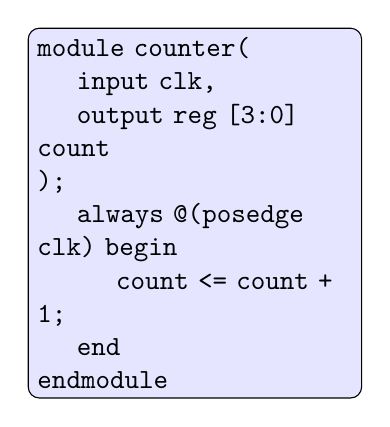
\begin{tikzpicture}
\node[draw, rounded corners, fill=blue!10, text width=4cm, align=left] {
\texttt{module counter(\\
\hspace*{0.5cm}input clk,\\
\hspace*{0.5cm}output reg [3:0] count\\
);\\
\hspace*{0.5cm}always @(posedge clk) begin\\
\hspace*{1cm}count <= count + 1;\\
\hspace*{0.5cm}end\\
endmodule}
};
\end{tikzpicture}
\end{minipage}
\end{center}

\column{0.55\textwidth}
\textbf{Simplified AST:}
\begin{center}
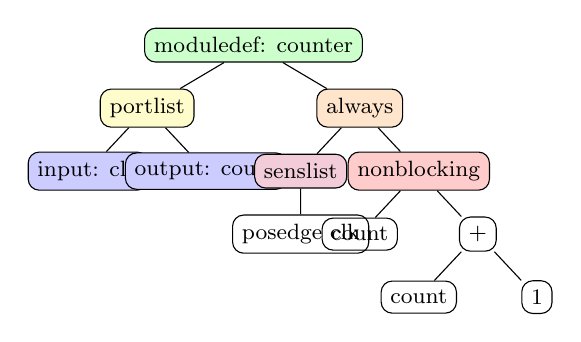
\begin{tikzpicture}[
    level distance=0.8cm,
    level 1/.style={sibling distance=2.7cm},
    level 2/.style={sibling distance=1.5cm},
    every node/.style={draw, rounded corners, font=\footnotesize}
]
\node[fill=green!20] {moduledef: counter}
    child {node[fill=yellow!20] {portlist}
        child {node[fill=blue!20] {input: clk}}
        child {node[fill=blue!20] {output: count}}
    }
    child {node[fill=orange!20] {always}
        child {node[fill=purple!20] {senslist}
            child {node {posedge clk}}
        }
        child {node[fill=red!20] {nonblocking}
            child {node {count}}
            child {node {+}
                child {node {count}}
                child {node {1}}
            }
        }
    };
\end{tikzpicture}
\end{center}
\end{columns}
\end{frame}

\begin{frame}
\frametitle{AST Node Types Discovered}
\begin{itemize}
    \item Our system discovered many Verilog constructs:
    \item Common node types:
    \begin{columns}
        \column{0.5\textwidth}
        \begin{itemize}
            \item \texttt{moduledef} (module definitions)
            \item \texttt{always} (always blocks)
            \item \texttt{senslist} (sensitivity lists)
            \item \texttt{if}/\texttt{case} (conditionals)
            \item \texttt{blocking}/\texttt{nonblocking} (assignments)
        \end{itemize}
        
        \column{0.5\textwidth}
        \begin{itemize}
            \item \texttt{rvalue}/\texttt{lvalue} (values)
            \item \texttt{pointer} (variable references)
            \item \texttt{eq}/\texttt{and}/\texttt{xor} (operators)
            \item \texttt{partselect} (bit selection)
            \item \texttt{concat} (concatenation)
        \end{itemize}
    \end{columns}
    \item Found 45+ unique node types across all samples
\end{itemize}
\end{frame}

\begin{frame}
\frametitle{Sample Type Dictionary from Processing}
\begin{columns}
\column{0.5\textwidth}
\begin{itemize}
    \item 0: source
    \item 1: description
    \item 2: moduledef
    \item 3: paramlist
    \item 4: portlist
    \item 5: decl
    \item 6: instancelist
    \item 7: ioport
    \item 8: input
    \item 9: width
    \item 10: intconst
    \item ...
\end{itemize}

\column{0.5\textwidth}
\begin{itemize}
    \item 19: block
    \item 20: sens
    \item 21: if
    \item 22: eq
    \item 23: nonblocking
    \item 24: lvalue
    \item 25: rvalue
    \item 26: pointer
    \item 27: xor
    \item 28: land
    \item ...
\end{itemize}
\end{columns}

\textbf{Each node type is assigned a unique ID for feature encoding}
\end{frame}

\begin{frame}
\frametitle{AST Feature Extraction}
Our system creates rich node features from AST:


\textbf{Process:} Verilog Code → Parse into AST → Convert to Graph → Extract Features

\begin{itemize}
    \item \textbf{Type encoding}: One-hot encoding of node type (50 dimensions)
    \item \textbf{Structural features}:
    \begin{itemize}
        \item Depth in AST (hierarchical position)
        \item Number of children (node complexity)
        \item Average child type ID (contextual information)
    \end{itemize}
    \item \textbf{Edge information}: Parent-child relationships
    \item These features capture both:
    \begin{itemize}
        \item Local code structure
        \item Global program patterns
    \end{itemize}
\end{itemize}
\end{frame}


\begin{frame}
\frametitle{Training Features: How We Represent AST Nodes}

\begin{columns}
\column{0.6\textwidth}
\textbf{Example Node Feature Vector:}
\begin{small}
\begin{tabular}{|l|c|}
\hline
\textbf{Feature Type} & \textbf{Value} \\
\hline
Type: moduledef & 1 (one-hot: [0,0,1,0,...]) \\
Depth in AST & 2 \\
Number of children & 5 \\
Average child type ID & 8.2 \\
\hline
\end{tabular}
\end{small}

\vspace{0.2cm}
\textbf{One-hot encoding example:}
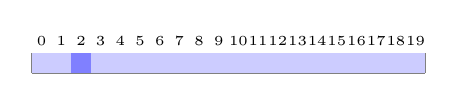
\begin{tikzpicture}
\draw[step=0.25cm,gray,very thin] (0,0) grid (5,0.25);
\foreach \x in {0,1,...,19} {
    \node[font=\tiny] at (\x*0.25+0.125,0.4) {\x};
}
\fill[blue!50] (0.5,0) rectangle (0.75,0.25);
\fill[blue!20] (0,0) rectangle (0.5,0.25);
\fill[blue!20] (0.75,0) rectangle (5,0.25);
\end{tikzpicture}


\column{0.4\textwidth}
\textbf{Why these features work:}
\begin{itemize}
    \item Type encoding captures node function
    \item Depth shows position in hierarchy
    \item Number of children indicates complexity
    \item Average child type provides context
\end{itemize}

\vspace{0.2cm}
\textbf{Full feature vector size:}
\begin{itemize}
    \item 50 dimensions for type (one-hot)
    \item 3 dimensions for structural info
    \item Total: 53+ dimensions
\end{itemize}
\end{columns}

\textbf{Sample from dataset:} A node from an "always" block in a trojan-infected circuit has different feature patterns than those in clean circuits.
\end{frame}

\section{GCN Architecture}

% \begin{frame}
% \frametitle{Understanding Graph Convolutional Networks (GCN)}

% \begin{columns}
% \column{0.5\textwidth}
% \textbf{What is a GCN?}
% \begin{itemize}
%     \item Neural network for graph data
%     \item Like CNN for images, but works on graphs
%     \item Learns patterns from connected nodes
% \end{itemize}

% \textbf{How does it work?}
% \begin{enumerate}
%     \item Each node collects information from its neighbors
%     \item Information is combined and transformed
%     \item Process repeats in layers
%     \item Final layer makes predictions
% \end{enumerate}

% \column{0.5\textwidth}
% \begin{tikzpicture}[
%     node/.style={circle, draw, minimum size=0.7cm},
%     arrow/.style={->, >=stealth, thick},
%     message/.style={->, >=stealth, dashed, red, thick}
% ]
% \node[node, fill=blue!20] (A) at (0,0) {A};
% \node[node, fill=green!20] (B) at (2,0) {B};
% \node[node, fill=yellow!20] (C) at (1,-1.5) {C};
% \node[node, fill=orange!20] (D) at (3,-1) {D};

% \draw (A) -- (B);
% \draw (A) -- (C);
% \draw (B) -- (C);
% \draw (B) -- (D);
% \draw (C) -- (D);

% \draw[message] (B) to[bend left=30] (A);
% \draw[message] (C) to[bend right=30] (A);
% \draw[message] (A) to[bend left=30] (B);
% \draw[message] (C) to[bend left=30] (B);
% \draw[message] (D) to[bend right=30] (B);

% \node[text width=4cm, align=center, font=\small] at (1.5,-2.5) {
%     Nodes exchange information with their neighbors
% };
% \end{tikzpicture}
% \end{columns}

% \textbf{Key insight}: GCNs can learn patterns in how code structures connect, helping identify suspicious patterns indicative of trojans.
% \end{frame}

% \begin{frame}
% \frametitle{How GCN Detects Hardware Trojans}

% \begin{columns}
% \column{0.5\textwidth}
% \begin{tikzpicture}[
%     box/.style={draw, rounded corners, minimum width=2.5cm, minimum height=0.7cm, align=center},
%     arrow/.style={->, >=stealth, thick}
% ]
% \node[box, fill=red!10] (ast1) at (0,0) {Trojan AST Pattern};
% \node[box, fill=green!10] (ast2) at (0,-1.5) {Normal AST Pattern};

% \begin{scope}[xshift=3.5cm]
%     \node[circle, draw, fill=red!10, minimum size=0.6cm] (n1) at (0,0) {};
%     \node[circle, draw, fill=red!10, minimum size=0.6cm] (n2) at (0.8,0.4) {};
%     \node[circle, draw, fill=red!10, minimum size=0.6cm] (n3) at (0.5,-0.7) {};
%     \node[circle, draw, fill=red!20, minimum size=0.6cm] (n4) at (1.2,-0.3) {};
%     \draw (n1) -- (n2);
%     \draw (n1) -- (n3);
%     \draw (n2) -- (n4);
%     \draw (n3) -- (n4);
% \end{scope}

% \begin{scope}[xshift=3.5cm, yshift=-1.5cm]
%     \node[circle, draw, fill=green!10, minimum size=0.6cm] (m1) at (0,0) {};
%     \node[circle, draw, fill=green!10, minimum size=0.6cm] (m2) at (0.8,0.4) {};
%     \node[circle, draw, fill=green!10, minimum size=0.6cm] (m3) at (0.5,-0.7) {};
%     \node[circle, draw, fill=green!10, minimum size=0.6cm] (m4) at (1.2,-0.3) {};
%     \draw (m1) -- (m2);
%     \draw (m1) -- (m3);
%     \draw (m2) -- (m4);
%     \draw (m3) -- (m4);
% \end{scope}

% \draw[arrow] (ast1) -- (n1);
% \draw[arrow] (ast2) -- (m1);
% \end{tikzpicture}

% \column{0.5\textwidth}
% \textbf{Common Trojan Patterns}:
% \begin{itemize}
%     \item Suspicious trigger conditions
%     \item Unusual signal connections
%     \item Redundant control logic
%     \item Rarely activated circuits
% \end{itemize}

% \textbf{GCN Learning Process}:
% \begin{enumerate}
%     \item Analyze node relationships
%     \item Recognize suspicious patterns
%     \item Compare to normal patterns
%     \item Classify as trojan/clean
% \end{enumerate}
% \end{columns}

% \vspace{0.3cm}
% \textbf{Real-world example}: GCN can identify when a signal is connected to an unusual part of the circuit or when rare trigger conditions are hidden in code.
% \end{frame}

\begin{frame}
\frametitle{What is a Graph Convolutional Network (GCN)?}

\begin{columns}
\column{0.5\textwidth}
\textbf{Simple definition:}
\begin{itemize}
    \item Neural network designed for graph data
    \item Learns patterns in connected data
    \item Like CNNs for images, but for graphs
\end{itemize}

 \item \textbf{Main operations}:
    \begin{itemize}
        \item Message passing between nodes
        \item Neighborhood aggregation
        \item Feature transformation
    \end{itemize}


\column{0.5\textwidth}
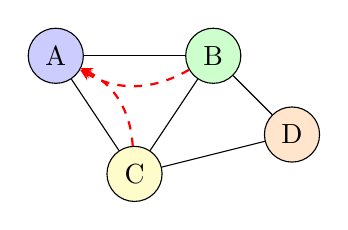
\begin{tikzpicture}[
    node/.style={circle, draw, minimum size=0.7cm},
    arrow/.style={->, >=stealth, thick},
    message/.style={->, >=stealth, dashed, red, thick}
]
\node[node, fill=blue!20] (A) at (0,0) {A};
\node[node, fill=green!20] (B) at (2,0) {B};
\node[node, fill=yellow!20] (C) at (1,-1.5) {C};
\node[node, fill=orange!20] (D) at (3,-1) {D};

\draw (A) -- (B);
\draw (A) -- (C);
\draw (B) -- (C);
\draw (B) -- (D);
\draw (C) -- (D);

\draw[message] (B) to[bend left=30] (A);
\draw[message] (C) to[bend right=30] (A);
\end{tikzpicture}

\textbf{Node A updates by receiving messages from neighbors B and C}
\end{columns}
\end{frame}

\begin{frame}
\frametitle{GCN: A Working Example}

\begin{columns}
\column{0.4\textwidth}
\textbf{Simple graph:}
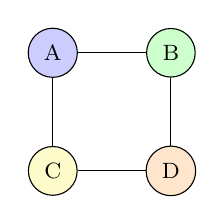
\begin{tikzpicture}[
    node/.style={circle, draw, minimum size=0.6cm, font=\footnotesize},
    arrow/.style={->, >=stealth}
]
\node[node, fill=blue!20] (A) at (0,0) {A};
\node[node, fill=green!20] (B) at (1.5,0) {B};
\node[node, fill=yellow!20] (C) at (0,-1.5) {C};
\node[node, fill=orange!20] (D) at (1.5,-1.5) {D};

\draw (A) -- (B);
\draw (A) -- (C);
\draw (B) -- (D);
\draw (C) -- (D);
\end{tikzpicture}

\textbf{Initial features:}
\begin{itemize}
    \item Node A: [1, 0]
    \item Node B: [0, 1]
    \item Node C: [1, 1]
    \item Node D: [0, 0]
\end{itemize}

\column{0.6\textwidth}
\textbf{GCN layer computation:}
\begin{enumerate}
    \item Each node collects neighbor features
    \item Apply weight matrix transformation
    \item Add non-linearity (ReLU)
\end{enumerate}

\textbf{Example for Node A:}
\begin{itemize}
    \item Initial feature: [1, 0]
    \item Neighbors: B, C
    \item Collect: [1, 0] + [0, 1] + [1, 1]
    \item Average: [0.67, 0.67]
    \item Apply weights: $W \cdot [0.67, 0.67]^T$
    \item Apply ReLU: max(0, result)
    \item New feature: [0.8, 1.2]
\end{itemize}
\end{columns}

\textbf{Over multiple layers, nodes gather information from wider neighborhoods}
\end{frame}


\begin{frame}
\frametitle{GNN Implementation: Complete Architecture}

\begin{columns}
\column{0.5\textwidth}
\begin{tikzpicture}[
    box/.style={draw, rounded corners, minimum width=3cm, minimum height=0.6cm, align=center, font=\footnotesize},
    smallbox/.style={draw, rounded corners, minimum width=2cm, minimum height=0.5cm, align=center, font=\scriptsize},
    arrow/.style={->, >=stealth, thick}
]
\node[box, fill=blue!10] (input) at (0,0) {Input: Graph with node features};
\node[smallbox, fill=purple!10, right=0.1cm of input] {x: 53+ dims};

\node[box, fill=green!10] (conv1) at (0,-1) {GCNConv Layer 1 (64 units)};
\node[smallbox, fill=orange!10, right=0.1cm of conv1] {ReLU};
\node[smallbox, fill=red!10, right=0.1cm of conv1, yshift=-0.6cm] {Dropout 0.5};

\node[box, fill=green!10] (conv2) at (0,-2.2) {GCNConv Layer 2 (64 units)};
\node[smallbox, fill=orange!10, right=0.1cm of conv2] {ReLU};
\node[smallbox, fill=red!10, right=0.1cm of conv2, yshift=-0.6cm] {Dropout 0.5};

\node[box, fill=yellow!10] (pool) at (0,-3.4) {Global Mean Pooling};
\node[box, fill=cyan!10] (linear) at (0,-4.2) {Linear Layer (64→1)};
\node[smallbox, fill=purple!10, right=0.1cm of linear] {Sigmoid};

\node[box, fill=red!10] (output) at (0,-5) {Output: Trojan probability};

\draw[arrow] (input) -- (conv1);
\draw[arrow] (conv1) -- (conv2);
\draw[arrow] (conv2) -- (pool);
\draw[arrow] (pool) -- (linear);
\draw[arrow] (linear) -- (output);
\end{tikzpicture}

\column{0.5\textwidth}
\textbf{GCNConv Layer Operations:}
\begin{enumerate}
    \item Calculate normalized adjacency matrix
    \item Aggregate features from neighbors
    \item Apply weight matrix transformation
    \item Add non-linearity (ReLU)
\end{enumerate}

\vspace{0.3cm}
\textbf{Dropout (0.5):} Randomly zeroes 50\% of features during training to prevent overfitting

\vspace{0.3cm}
\textbf{Global Mean Pooling:} Averages all node features to get a single graph representation

\vspace{0.3cm}
\textbf{Loss Function:} Binary Cross Entropy with class weighting (0.26) to handle imbalance
\end{columns}
\end{frame}

\section{Experimental Results}

\begin{frame}
\frametitle{Dataset Statistics}
\begin{itemize}
    \item \textbf{Dataset}: TJ-RTL-toy benchmark
    \item \textbf{Total circuits}: 43
    \begin{itemize}
        \item 34 Trojan-infected (79\%)
        \item 9 Trojan-free (21\%)
    \end{itemize}
    \item \textbf{Class imbalance}: 0.26:1 (Clean:Trojan)
    \item \textbf{Circuits processed}:
    \begin{itemize}
        \item AES, RC5, RC6, PIC16F84, RS232, VGA, XTEA, etc.
    \end{itemize}
    \item \textbf{Node types discovered}: 45+
\end{itemize}
\end{frame}

\begin{frame}
\frametitle{Experimental Setup}
\begin{itemize}
    \item \textbf{Cross-validation}: 2-fold stratified
    \item \textbf{Oversampling}: Random oversampling of minority class
    \item \textbf{Training}:
    \begin{itemize}
        \item 100 epochs
        \item Adam optimizer (lr=0.001)
        \item BCELoss with class weighting
        \item Batch size: 32
    \end{itemize}
    \item \textbf{Model}: GCN with 2 layers (64 hidden units)
    \item \textbf{Random seed}: 42 (for reproducibility)
\end{itemize}
\end{frame}

\begin{frame}
\frametitle{Implementation Details}

\begin{columns}

\column{0.33\textwidth}
\textbf{Key Libraries:}
\begin{itemize}
    \item \textbf{PyTorch} (v1.10+)
    \item \textbf{PyTorch Geometric} (PyG)
    \item \textbf{PyVerilog} parser
    \item \textbf{NetworkX} for graphs
    \item \textbf{NumPy/Scikit-learn}
    \item \textbf{Matplotlib}
\end{itemize}

\textbf{GNN Components:}
\begin{itemize}
    \item \texttt{GCNConv} (primary)
    \item \texttt{global\_mean\_pool}
\end{itemize}


\column{0.33\textwidth}
\vspace{-0.5em} % Optional: reduce vertical space
\textbf{Hardware/Runtime:}
\begin{itemize}
    \item \textbf{GPU}: NVIDIA RTX 3060 mobile
    \item \textbf{Training Time}: ~30s
    \item \textbf{Codebase}: Python 3.9
\end{itemize}

\end{columns}

\end{frame}

\begin{frame}
\frametitle{Performance Metrics}
\begin{table}
\centering
\begin{tabular}{lcc|c}
\toprule
\textbf{Metric} & \textbf{Fold 1} & \textbf{Fold 2} & \textbf{Average} \\
\midrule
Accuracy & 0.5909 & 0.9048 & 0.7478 \\
Precision & 0.9000 & 1.0000 & 0.9500 \\
Recall & 0.5294 & 0.8824 & 0.7059 \\
F1 Score & 0.6667 & 0.9375 & 0.8021 \\
\bottomrule
\end{tabular}
\caption{Performance metrics across folds}
\end{table}

\begin{table}
\centering
\begin{tabular}{cc|cc}
\multicolumn{4}{c}{\textbf{Average Confusion Matrix}} \\
\multicolumn{2}{c}{} & \multicolumn{2}{c}{\textbf{Predicted}} \\
& & \textbf{Clean} & \textbf{Trojan} \\
\cmidrule{3-4}
\multirow{2}{*}{\textbf{Actual}} & \textbf{Clean} & 4.0 & 0.5 \\
& \textbf{Trojan} & 5.0 & 12.0 \\
\end{tabular}
\end{table}
\end{frame}

\begin{frame}
\frametitle{Key Findings}
\begin{itemize}
    \item \textbf{High precision} (95\%): Few false positives
    \item \textbf{Good F1 score} (80.2\%): Balanced performance
    \item \textbf{Improvement across folds}: Fold 2 significantly better
\end{itemize}
\end{frame}

\begin{frame}
\frametitle{Discussion \& Limitations}
\begin{itemize}
    \item \textbf{Strengths}:
    \begin{itemize}
        \item High precision - few false positives
        \item Effective at capturing code-level trojans
    \end{itemize}
    \item \textbf{Limitations}:
    \begin{itemize}
        \item Small dataset (43 circuits)
        \item Class imbalance (more trojans than clean)
        \item Fold variation indicates potential overfitting
    \end{itemize}
    \item \textbf{Future work}: Larger datasets, more complex architectures
\end{itemize}
\end{frame}

\begin{frame}
\frametitle{Conclusions: What We've Learned}

\begin{columns}
\column{0.5\textwidth}
\textbf{Key achievements:}
\begin{itemize}
    \item Used code structure (AST) 
    \item Achieved 75\% accuracy, 95\% precision
\end{itemize}



\column{0.5\textwidth}
\textbf{Next steps:}
\begin{itemize}
    \item Larger, more diverse datasets
    \item Hyperparameter optimization 
    \item Hybrid architecture (GNN+MLP)
    \item Neural architecture search
    

\end{itemize}
\end{columns}
\end{frame}

\begin{frame}
\frametitle{Thank You!}
\begin{center}
\Huge Questions?
\end{center}
\end{frame}

\end{document}